Limits are important in calculus since we need very small quantities to effectively study change. Yeah, that's pretty vague, but hopefully it'll clear up in a few pages.

We study limits for many reasons. One of them is to study functions at points where they are only ``close'' to being defined. Another is to make quantities very (arbitrarily) small, without making them 0.

Here is an example of a practical use of limits. The following two functions' graphs are exactly the same, except at $x=1$.

\begin{figure}[h!]
    \centering
    \fbox{
    \resizebox{4in}{!}{


\tikzset{every picture/.style={line width=0.75pt}} %set default line width to 0.75pt        

\begin{tikzpicture}[x=0.75pt,y=0.75pt,yscale=-1,xscale=1]
%uncomment if require: \path (0,300); %set diagram left start at 0, and has height of 300

%Straight Lines [id:da5436445771795901] 
\draw  [dash pattern={on 0.84pt off 2.51pt}]  (392,151.33) -- (318,151.17) ;
%Straight Lines [id:da6949730842855149] 
\draw  [dash pattern={on 0.84pt off 2.51pt}]  (392,151.33) -- (392,219.5) ;
%Straight Lines [id:da8209687086477877] 
\draw    (49,79.83) -- (49,231.5) ;
%Curve Lines [id:da9233668280128751] 
\draw    (41,186.5) .. controls (59,138.83) and (98,184.83) .. (123,152.83) ;
%Curve Lines [id:da7989009557315903] 
\draw    (123,152.83) .. controls (150,110.83) and (183,173.83) .. (223,143.83) ;

%Straight Lines [id:da6182960293771871] 
\draw    (233,221) -- (39,221) ;
%Straight Lines [id:da04200773563301774] 
\draw    (317,79.83) -- (317,231.5) ;
%Straight Lines [id:da726566232707935] 
\draw    (501,220.5) -- (307,220.5) ;
%Curve Lines [id:da20535665951890536] 
\draw    (309,186.5) .. controls (327,138.83) and (366,184.83) .. (391,152.83) ;
%Curve Lines [id:da8509447981009293] 
\draw    (391,152.83) .. controls (418,110.83) and (451,173.83) .. (491,143.83) ;
%Shape: Circle [id:dp8197107597318569] 
\draw  [fill={rgb, 255:red, 255; green, 255; blue, 255 }  ,fill opacity=1 ] (388.5,151.33) .. controls (388.5,149.4) and (390.07,147.83) .. (392,147.83) .. controls (393.93,147.83) and (395.5,149.4) .. (395.5,151.33) .. controls (395.5,153.27) and (393.93,154.83) .. (392,154.83) .. controls (390.07,154.83) and (388.5,153.27) .. (388.5,151.33) -- cycle ;

%Straight Lines [id:da7228354618576209] 
\draw  [dash pattern={on 0.84pt off 2.51pt}]  (123,152.83) -- (123,221) ;
%Straight Lines [id:da24003054824236258] 
\draw  [dash pattern={on 0.84pt off 2.51pt}]  (123,152.83) -- (49,152.67) ;

% Text Node
\draw (119,227.4) node [anchor=north west][inner sep=0.75pt]    {$1$};
% Text Node
\draw (388.5,227.4) node [anchor=north west][inner sep=0.75pt]    {$1$};
% Text Node
\draw (26,145) node [anchor=north west][inner sep=0.75pt]    {$10$};
% Text Node
\draw (294,145) node [anchor=north west][inner sep=0.75pt]    {$10$};


\end{tikzpicture}

    }}
    \caption{Two functions with the same limits}
\end{figure}

The first function is defined at $x=1$, while the second function is not. However, the values of the second function are near 10 when $x$ is near 1. There is still something useful we can say about the second function at 1: ``the \textit{limit} at 1 is 10.''



\section{Definitions}

\subsection{The Limit}

The intuitive idea of a \textbf{limit} is to examine what the output of a function does as the input moves close to a specific value. We say that the limit of $f$ at $a$ is $L$ if $f(x)$ moves closer to $L$ as as $x$ moves closer to $a$. Note that $f$ need not be defined at $a$ to find the limit of $f$ as $x$ approaches $a$ (in fact, that's the whole point!).

Since the functions we care about take real numbers as inputs, there are two ways you can approach a number on the real line (from the left and from the right). We will talk about left- and right-sided limits.

If $f$ is defined on an interval to the \textit{left} of $a$ (with $a$ as an endpoint) and the values of $f(x)$ approach $L$ as $x$ approaches $a$ from the \textit{left}, we say that the ``\textbf{left-sided limit of $f$ as $x$ approaches $a$} is $L$'' and we write $$\lim_{x\to a^-}f(x)=L.$$
If $f$ is defined on an interval to the \textit{right} of $a$ (with $a$ as an endpoint) and the values of $f(x)$ approach $L$ as $x$ approaches $a$ from the \textit{right}, we say that the \textbf{right-sided limit of $f$ as $x$ approaches $a$} is $L$'' and we write
$$\lim_{x\to a^+}f(x)=L.$$
If the right and left sided limits match, then we say that the \textbf{limit of $f$ as $x$ approaches $a$ is $L$} and write $$\lim_{x\to a}f(x)=L.$$

If the left and right sided limits, do not match, then we say that the limit \textbf{does not exist} (DNE).

One can compute $f(x)$ for values of $x$ that get closer and closer to either side of $a$. If the values approach $L$, then you have good reason to believe that $L$ is the (right- and/or left-sided) limit.

\begin{center}
\begin{tabular}{@{}ll@{}}
\toprule[0.4mm]
   $x$        & $f(x)$        \\
\midrule
   $a-0.1$    & $f(a-0.1)$    \\
   $a-0.01$   & $f(a-0.01)$   \\
   $a-0.001$  & $f(a-0.001)$  \\
   $a-0.0001$ & $f(a-0.0001)$ \\
\midrule
   $a+0.0001$ & $f(a+0.0001)$ \\
   $a+0.001$  & $f(a+0.001)$  \\
   $a+0.01$   & $f(a+0.01)$   \\
   $a+0.1$    & $f(a+0.1)$    \\
\bottomrule[0.4mm]
\end{tabular}
\end{center}
Such calculations, however, cannot prove that a function limits to a specific value.


\subsection{Infinite Limits}

We can extend the idea of limits outside of the real numbers to include positive and negative infinity in place of both $a$ and $L$.
\begin{itemize}
\item If $f(x)$ grows without bound as $x$ approaches $a$ from the left, then we write $$\lim_{x\to a^-}f(x)=\infty.$$
(Similarly for $x$ approaching $a$ from the right, and also if $f(x)$ becomes increasingly negative without bound).
\item We denote the value (if such a value exists) that $f(x)$ approaches as $x$ approaches $\infty$ as $$\lim_{x\to\infty} f(x).$$
(Similarly if $x$ approaches $-\infty$).
\end{itemize}


\subsection{Optional: The $\varepsilon-\delta$ Definition}

You may be dissatisfied with the intuitive approach to limits, so we can make the definition more rigorous. The main idea that needs to be captured by a formal definition is \textit{arbitrary precision}. That is, we need a way to say formally that ``$f(x)$ approaches $L$ as $x$ approaches $a$.''

By controlling the input $x$, we must be able to make the distance $|f(x)-L|$ between the output $f(x)$ and $L$ to be as small as we want (``arbitrarily small''). In other words, if $\varepsilon>0$ is any small positive number, we must be able to ensure (by controlling $x$) that $|f(x)-L| < \varepsilon$. To control $x$, we can make the distance $|x-a|$ between $x$ and $a$ smaller than some positive number $\delta > 0$ (that may depend on $\varepsilon$).

Now we're ready for the real ``$\varepsilon-\delta$'' definition of a limit: we say that \textbf{$L$ is the limit of $f$ as $x$ approaches $a$} if
$$\text{for all } \varepsilon > 0, \text{ there is some } \delta > 0, \text{ such that } |x - a| < \delta \implies |f(x) - L| <\varepsilon.$$

\mar{Read that definition a few times, because statements with multiple quantifiers can be tricky!}

\begin{figure}[h!]
\centering
\fbox{
\tikzset{every picture/.style={line width=0.75pt}}
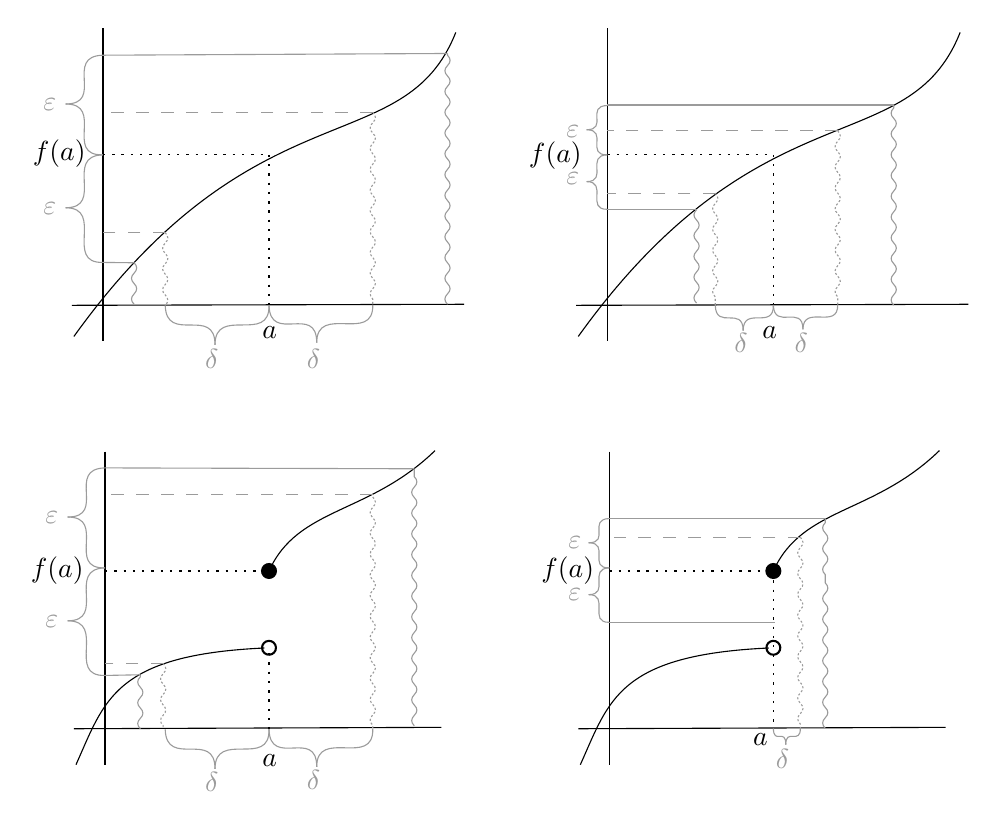
\begin{tikzpicture}[x=0.75pt,y=0.75pt,yscale=-1,xscale=1]
%uncomment if require: \path (0,428); %set diagram left start at 0, and has height of 428

%Straight Lines [id:da2730924968926851]
\draw    (71,155) -- (260,154.5) ;
%Straight Lines [id:da38663844155403493]
\draw    (86,21.5) -- (86,172.33) ;
%Curve Lines [id:da5832897062677318]
\draw    (72,170) .. controls (160,47.5) and (231,86.5) .. (256,23.5) ;
%Curve Lines [id:da15926967534570857]
\draw    (73,376.33) .. controls (86.86,345.64) and (90.92,323.45) .. (163.77,320.1) ;
\draw [shift={(166,320)}, rotate = 357.71] [color={rgb, 255:red, 0; green, 0; blue, 0 }  ][line width=0.75]      (0, 0) circle [x radius= 3.35, y radius= 3.35]   ;
%Curve Lines [id:da573129079856388]
\draw    (166,283) .. controls (180,252) and (214,256) .. (246,225) ;
\draw [shift={(166,283)}, rotate = 294.3] [color={rgb, 255:red, 0; green, 0; blue, 0 }  ][fill={rgb, 255:red, 0; green, 0; blue, 0 }  ][line width=0.75]      (0, 0) circle [x radius= 3.35, y radius= 3.35]   ;
%Straight Lines [id:da06544192635535961]
\draw  [dash pattern={on 0.84pt off 2.51pt}]  (166,82.5) -- (166,154.92) ;
%Straight Lines [id:da8462520068785757]
\draw  [dash pattern={on 0.84pt off 2.51pt}]  (86,82.5) -- (166,82.5) ;
%Straight Lines [id:da8033956316212987]
\draw [color={rgb, 255:red, 155; green, 155; blue, 155 }  ,draw opacity=1 ]   (86,34.5) -- (252,33.67) ;
%Straight Lines [id:da9058328806059841]
\draw [color={rgb, 255:red, 155; green, 155; blue, 155 }  ,draw opacity=1 ]   (86,134.33) -- (101,134.5) ;
%Straight Lines [id:da7683874289412185]
\draw    (72,359) -- (249,358.33) ;
%Straight Lines [id:da21021021460529377]
\draw    (87,225.5) -- (87,376.33) ;
%Straight Lines [id:da5263630709862186]
\draw  [dash pattern={on 0.84pt off 2.51pt}]  (166,322.58) -- (166,359.25) ;
%Straight Lines [id:da2255352189878881]
\draw  [dash pattern={on 0.84pt off 2.51pt}]  (87,283) -- (166,283) ;
%Straight Lines [id:da12241776303117424]
\draw [color={rgb, 255:red, 155; green, 155; blue, 155 }  ,draw opacity=1 ]   (87,233.33) -- (236,233.75) ;
%Straight Lines [id:da6551551228954233]
\draw [color={rgb, 255:red, 155; green, 155; blue, 155 }  ,draw opacity=1 ]   (87,333.33) -- (104,333) ;
%Straight Lines [id:da3470258564776276]
\draw [color={rgb, 255:red, 155; green, 155; blue, 155 }  ,draw opacity=1 ] [dash pattern={on 0.75pt off 0.75pt}]  (116,120) .. controls (117.67,121.67) and (117.67,123.33) .. (116,125) .. controls (114.33,126.67) and (114.33,128.33) .. (116,130) .. controls (117.67,131.67) and (117.67,133.33) .. (116,135) .. controls (114.33,136.67) and (114.33,138.33) .. (116,140) .. controls (117.67,141.67) and (117.67,143.33) .. (116,145) .. controls (114.33,146.67) and (114.33,148.33) .. (116,150) .. controls (117.67,151.67) and (117.67,153.33) .. (116,155) -- (116,155) ;
%Straight Lines [id:da2371091562631653]
\draw [color={rgb, 255:red, 155; green, 155; blue, 155 }  ,draw opacity=1 ] [dash pattern={on 0.75pt off 0.75pt}]  (216,62) .. controls (217.67,63.67) and (217.67,65.33) .. (216,67) .. controls (214.33,68.67) and (214.33,70.33) .. (216,72) .. controls (217.67,73.67) and (217.67,75.33) .. (216,77) .. controls (214.33,78.67) and (214.33,80.33) .. (216,82) .. controls (217.67,83.67) and (217.67,85.33) .. (216,87) .. controls (214.33,88.67) and (214.33,90.33) .. (216,92) .. controls (217.67,93.67) and (217.67,95.33) .. (216,97) .. controls (214.33,98.67) and (214.33,100.33) .. (216,102) .. controls (217.67,103.67) and (217.67,105.33) .. (216,107) .. controls (214.33,108.67) and (214.33,110.33) .. (216,112) .. controls (217.67,113.67) and (217.67,115.33) .. (216,117) .. controls (214.33,118.67) and (214.33,120.33) .. (216,122) .. controls (217.67,123.67) and (217.67,125.33) .. (216,127) .. controls (214.33,128.67) and (214.33,130.33) .. (216,132) .. controls (217.67,133.67) and (217.67,135.33) .. (216,137) .. controls (214.33,138.67) and (214.33,140.33) .. (216,142) .. controls (217.67,143.67) and (217.67,145.33) .. (216,147) .. controls (214.33,148.67) and (214.33,150.33) .. (216,152) -- (216,154.71) -- (216,154.71) ;
%Straight Lines [id:da47940446384008517]
\draw [color={rgb, 255:red, 155; green, 155; blue, 155 }  ,draw opacity=1 ] [dash pattern={on 4.5pt off 4.5pt}]  (116,120) -- (86,120) ;
%Straight Lines [id:da2718218581855085]
\draw [color={rgb, 255:red, 155; green, 155; blue, 155 }  ,draw opacity=1 ] [dash pattern={on 4.5pt off 4.5pt}]  (216,62) -- (86,62) ;
%Curve Lines [id:da7867325499156288]
\draw [color={rgb, 255:red, 155; green, 155; blue, 155 }  ,draw opacity=1 ]   (68,58) .. controls (87,58) and (67,35) .. (86,34.5) ;
%Curve Lines [id:da8389021578247982]
\draw [color={rgb, 255:red, 155; green, 155; blue, 155 }  ,draw opacity=1 ]   (68,58) .. controls (87,58) and (67,83) .. (86,82.5) ;
%Curve Lines [id:da6940267896547274]
\draw [color={rgb, 255:red, 155; green, 155; blue, 155 }  ,draw opacity=1 ]   (68,108) .. controls (87,108) and (67,83) .. (86,82.5) ;
%Curve Lines [id:da9368251006708403]
\draw [color={rgb, 255:red, 155; green, 155; blue, 155 }  ,draw opacity=1 ]   (68,108) .. controls (87,108) and (67,134.83) .. (86,134.33) ;
%Curve Lines [id:da7416463958304471]
\draw [color={rgb, 255:red, 155; green, 155; blue, 155 }  ,draw opacity=1 ]   (139.99,174) .. controls (140,155) and (116.5,174) .. (116,155) ;
%Curve Lines [id:da0946019041451891]
\draw [color={rgb, 255:red, 155; green, 155; blue, 155 }  ,draw opacity=1 ]   (139.99,174) .. controls (140,155) and (166.5,173.92) .. (166,154.92) ;
%Curve Lines [id:da8479225025412045]
\draw [color={rgb, 255:red, 155; green, 155; blue, 155 }  ,draw opacity=1 ]   (188.99,173) .. controls (189,154) and (166.5,173.92) .. (166,154.92) ;
%Curve Lines [id:da5287374586288269]
\draw [color={rgb, 255:red, 155; green, 155; blue, 155 }  ,draw opacity=1 ]   (188.99,173) .. controls (189,154) and (216.5,173.71) .. (216,154.71) ;
%Straight Lines [id:da5763369512697336]
\draw [color={rgb, 255:red, 155; green, 155; blue, 155 }  ,draw opacity=1 ]   (101,154.5) .. controls (99.33,152.83) and (99.33,151.17) .. (101,149.5) .. controls (102.67,147.83) and (102.67,146.17) .. (101,144.5) .. controls (99.33,142.83) and (99.33,141.17) .. (101,139.5) .. controls (102.67,137.83) and (102.67,136.17) .. (101,134.5) -- (101,134.5) ;
%Straight Lines [id:da9925497456851824]
\draw [color={rgb, 255:red, 155; green, 155; blue, 155 }  ,draw opacity=1 ]   (252,154.5) .. controls (250.33,152.83) and (250.33,151.17) .. (252,149.5) .. controls (253.67,147.83) and (253.67,146.17) .. (252,144.5) .. controls (250.33,142.83) and (250.33,141.17) .. (252,139.5) .. controls (253.67,137.83) and (253.67,136.17) .. (252,134.5) .. controls (250.33,132.83) and (250.33,131.17) .. (252,129.5) .. controls (253.67,127.83) and (253.67,126.17) .. (252,124.5) .. controls (250.33,122.83) and (250.33,121.17) .. (252,119.5) .. controls (253.67,117.83) and (253.67,116.17) .. (252,114.5) .. controls (250.33,112.83) and (250.33,111.17) .. (252,109.5) .. controls (253.67,107.83) and (253.67,106.17) .. (252,104.5) .. controls (250.33,102.83) and (250.33,101.17) .. (252,99.5) .. controls (253.67,97.83) and (253.67,96.17) .. (252,94.5) .. controls (250.33,92.83) and (250.33,91.17) .. (252,89.5) .. controls (253.67,87.83) and (253.67,86.17) .. (252,84.5) .. controls (250.33,82.83) and (250.33,81.17) .. (252,79.5) .. controls (253.67,77.83) and (253.67,76.17) .. (252,74.5) .. controls (250.33,72.83) and (250.33,71.17) .. (252,69.5) .. controls (253.67,67.83) and (253.67,66.17) .. (252,64.5) .. controls (250.33,62.83) and (250.33,61.17) .. (252,59.5) .. controls (253.67,57.83) and (253.67,56.17) .. (252,54.5) .. controls (250.33,52.83) and (250.33,51.17) .. (252,49.5) .. controls (253.67,47.83) and (253.67,46.17) .. (252,44.5) .. controls (250.33,42.83) and (250.33,41.17) .. (252,39.5) .. controls (253.67,37.83) and (253.67,36.17) .. (252,34.5) -- (252,33.67) -- (252,33.67) ;
%Curve Lines [id:da7131476230234577]
\draw [color={rgb, 255:red, 155; green, 155; blue, 155 }  ,draw opacity=1 ]   (69,257) .. controls (88,257) and (68,233.83) .. (87,233.33) ;
%Curve Lines [id:da5212410455410692]
\draw [color={rgb, 255:red, 155; green, 155; blue, 155 }  ,draw opacity=1 ]   (69,257) .. controls (88,257) and (68,282) .. (87,281.5) ;
%Curve Lines [id:da8037674418363849]
\draw [color={rgb, 255:red, 155; green, 155; blue, 155 }  ,draw opacity=1 ]   (69,307) .. controls (88,307) and (68,282) .. (87,281.5) ;
%Curve Lines [id:da3061502012065347]
\draw [color={rgb, 255:red, 155; green, 155; blue, 155 }  ,draw opacity=1 ]   (69,307) .. controls (88,307) and (68,333.83) .. (87,333.33) ;
%Curve Lines [id:da838846723146208]
\draw [color={rgb, 255:red, 155; green, 155; blue, 155 }  ,draw opacity=1 ]   (139.99,378.34) .. controls (140,359.34) and (116.5,378.33) .. (116,359.33) ;
%Curve Lines [id:da45926415056497105]
\draw [color={rgb, 255:red, 155; green, 155; blue, 155 }  ,draw opacity=1 ]   (139.99,378.34) .. controls (140,359.34) and (166.5,378.25) .. (166,359.25) ;
%Curve Lines [id:da1812164249288335]
\draw [color={rgb, 255:red, 155; green, 155; blue, 155 }  ,draw opacity=1 ]   (188.99,377.34) .. controls (189,358.34) and (166.5,378.25) .. (166,359.25) ;
%Curve Lines [id:da5310165714599331]
\draw [color={rgb, 255:red, 155; green, 155; blue, 155 }  ,draw opacity=1 ]   (188.99,377.34) .. controls (189,358.34) and (216.5,378.04) .. (216,359.04) ;
%Straight Lines [id:da1373743464903565]
\draw [color={rgb, 255:red, 155; green, 155; blue, 155 }  ,draw opacity=1 ] [dash pattern={on 0.75pt off 0.75pt}]  (115,327.5) .. controls (116.67,329.17) and (116.67,330.83) .. (115,332.5) .. controls (113.33,334.17) and (113.33,335.83) .. (115,337.5) .. controls (116.67,339.17) and (116.67,340.83) .. (115,342.5) .. controls (113.33,344.17) and (113.33,345.83) .. (115,347.5) .. controls (116.67,349.17) and (116.67,350.83) .. (115,352.5) .. controls (113.33,354.17) and (113.33,355.83) .. (115,357.5) -- (115,359) -- (115,359) ;
%Straight Lines [id:da30273639101181327]
\draw [color={rgb, 255:red, 155; green, 155; blue, 155 }  ,draw opacity=1 ] [dash pattern={on 0.75pt off 0.75pt}]  (216,247.33) .. controls (217.67,249) and (217.67,250.66) .. (216,252.33) .. controls (214.33,254) and (214.33,255.66) .. (216,257.33) .. controls (217.67,259) and (217.67,260.66) .. (216,262.33) .. controls (214.33,264) and (214.33,265.66) .. (216,267.33) .. controls (217.67,269) and (217.67,270.66) .. (216,272.33) .. controls (214.33,274) and (214.33,275.66) .. (216,277.33) .. controls (217.67,279) and (217.67,280.66) .. (216,282.33) .. controls (214.33,284) and (214.33,285.66) .. (216,287.33) .. controls (217.67,289) and (217.67,290.66) .. (216,292.33) .. controls (214.33,294) and (214.33,295.66) .. (216,297.33) .. controls (217.67,299) and (217.67,300.66) .. (216,302.33) .. controls (214.33,304) and (214.33,305.66) .. (216,307.33) .. controls (217.67,309) and (217.67,310.66) .. (216,312.33) .. controls (214.33,314) and (214.33,315.66) .. (216,317.33) .. controls (217.67,319) and (217.67,320.66) .. (216,322.33) .. controls (214.33,324) and (214.33,325.66) .. (216,327.33) .. controls (217.67,329) and (217.67,330.66) .. (216,332.33) .. controls (214.33,334) and (214.33,335.66) .. (216,337.33) .. controls (217.67,339) and (217.67,340.66) .. (216,342.33) .. controls (214.33,344) and (214.33,345.66) .. (216,347.33) .. controls (217.67,349) and (217.67,350.66) .. (216,352.33) .. controls (214.33,354) and (214.33,355.66) .. (216,357.33) -- (216,359.04) -- (216,359.04) ;
%Straight Lines [id:da6690760580285089]
\draw [color={rgb, 255:red, 155; green, 155; blue, 155 }  ,draw opacity=1 ] [dash pattern={on 4.5pt off 4.5pt}]  (115,327.5) -- (87,327.5) ;
%Straight Lines [id:da023392902319420816]
\draw [color={rgb, 255:red, 155; green, 155; blue, 155 }  ,draw opacity=1 ] [dash pattern={on 4.5pt off 4.5pt}]  (216,246) -- (87,246) ;
%Straight Lines [id:da7002803226646901]
\draw [color={rgb, 255:red, 155; green, 155; blue, 155 }  ,draw opacity=1 ]   (104,359) .. controls (102.33,357.33) and (102.33,355.67) .. (104,354) .. controls (105.67,352.33) and (105.67,350.67) .. (104,349) .. controls (102.33,347.33) and (102.33,345.67) .. (104,344) .. controls (105.67,342.33) and (105.67,340.67) .. (104,339) .. controls (102.33,337.33) and (102.33,335.67) .. (104,334) -- (104,333) -- (104,333) ;
%Straight Lines [id:da5440309336359443]
\draw [color={rgb, 255:red, 155; green, 155; blue, 155 }  ,draw opacity=1 ]   (236,357.58) .. controls (234.33,355.91) and (234.33,354.25) .. (236,352.58) .. controls (237.67,350.91) and (237.67,349.25) .. (236,347.58) .. controls (234.33,345.91) and (234.33,344.25) .. (236,342.58) .. controls (237.67,340.91) and (237.67,339.25) .. (236,337.58) .. controls (234.33,335.91) and (234.33,334.25) .. (236,332.58) .. controls (237.67,330.91) and (237.67,329.25) .. (236,327.58) .. controls (234.33,325.91) and (234.33,324.25) .. (236,322.58) .. controls (237.67,320.91) and (237.67,319.25) .. (236,317.58) .. controls (234.33,315.91) and (234.33,314.25) .. (236,312.58) .. controls (237.67,310.91) and (237.67,309.25) .. (236,307.58) .. controls (234.33,305.91) and (234.33,304.25) .. (236,302.58) .. controls (237.67,300.91) and (237.67,299.25) .. (236,297.58) .. controls (234.33,295.91) and (234.33,294.25) .. (236,292.58) .. controls (237.67,290.91) and (237.67,289.25) .. (236,287.58) .. controls (234.33,285.91) and (234.33,284.25) .. (236,282.58) .. controls (237.67,280.91) and (237.67,279.25) .. (236,277.58) .. controls (234.33,275.91) and (234.33,274.25) .. (236,272.58) .. controls (237.67,270.91) and (237.67,269.25) .. (236,267.58) .. controls (234.33,265.91) and (234.33,264.25) .. (236,262.58) .. controls (237.67,260.91) and (237.67,259.25) .. (236,257.58) .. controls (234.33,255.91) and (234.33,254.25) .. (236,252.58) .. controls (237.67,250.91) and (237.67,249.25) .. (236,247.58) .. controls (234.33,245.91) and (234.33,244.25) .. (236,242.58) .. controls (237.67,240.91) and (237.67,239.25) .. (236,237.58) -- (236,233.75) -- (236,233.75) ;

%Straight Lines [id:da8513462018635212]
\draw    (314,155) -- (503,154.5) ;
%Straight Lines [id:da27501056686778513]
\draw    (329,21.5) -- (329,172.33) ;
%Curve Lines [id:da5516996470591613]
\draw    (315,170) .. controls (403,47.5) and (474,86.5) .. (499,23.5) ;
%Curve Lines [id:da2905586367584121]
\draw    (316,376.33) .. controls (329.86,345.64) and (333.92,323.45) .. (406.77,320.1) ;
\draw [shift={(409,320)}, rotate = 357.71] [color={rgb, 255:red, 0; green, 0; blue, 0 }  ][line width=0.75]      (0, 0) circle [x radius= 3.35, y radius= 3.35]   ;
%Curve Lines [id:da17327963328411955]
\draw    (409,283) .. controls (423,252) and (457,256) .. (489,225) ;
\draw [shift={(409,283)}, rotate = 294.3] [color={rgb, 255:red, 0; green, 0; blue, 0 }  ][fill={rgb, 255:red, 0; green, 0; blue, 0 }  ][line width=0.75]      (0, 0) circle [x radius= 3.35, y radius= 3.35]   ;
%Straight Lines [id:da4442118515906792]
\draw  [dash pattern={on 0.84pt off 2.51pt}]  (409,82.5) -- (409,154.92) ;
%Straight Lines [id:da4615400041448172]
\draw  [dash pattern={on 0.84pt off 2.51pt}]  (329,82.5) -- (409,82.5) ;
%Straight Lines [id:da9140897903442382]
\draw [color={rgb, 255:red, 155; green, 155; blue, 155 }  ,draw opacity=1 ]   (329,58.5) -- (467,58.5) ;
%Straight Lines [id:da8879320022705979]
\draw [color={rgb, 255:red, 155; green, 155; blue, 155 }  ,draw opacity=1 ]   (329,108.73) -- (372,108.73) ;
%Straight Lines [id:da17895890987358554]
\draw    (315,359) -- (492,358.33) ;
%Straight Lines [id:da05857321637633417]
\draw    (330,225.5) -- (330,376.33) ;
%Straight Lines [id:da07307770178123163]
\draw  [dash pattern={on 0.84pt off 2.51pt}]  (409,283) -- (409,359.25) ;
%Straight Lines [id:da06234038795466201]
\draw  [dash pattern={on 0.84pt off 2.51pt}]  (330,283) -- (409,283) ;
%Straight Lines [id:da8599377579018705]
\draw [color={rgb, 255:red, 155; green, 155; blue, 155 }  ,draw opacity=1 ]   (330,257.73) -- (434,257.73) ;
%Straight Lines [id:da9417232436931344]
\draw [color={rgb, 255:red, 155; green, 155; blue, 155 }  ,draw opacity=1 ]   (330,307.73) -- (410,307.73) ;
%Straight Lines [id:da21280146915905584]
\draw [color={rgb, 255:red, 155; green, 155; blue, 155 }  ,draw opacity=1 ] [dash pattern={on 0.75pt off 0.75pt}]  (381,100.93) .. controls (382.67,102.6) and (382.67,104.26) .. (381,105.93) .. controls (379.33,107.6) and (379.33,109.26) .. (381,110.93) .. controls (382.67,112.6) and (382.67,114.26) .. (381,115.93) .. controls (379.33,117.6) and (379.33,119.26) .. (381,120.93) .. controls (382.67,122.6) and (382.67,124.26) .. (381,125.93) .. controls (379.33,127.6) and (379.33,129.26) .. (381,130.93) .. controls (382.67,132.6) and (382.67,134.26) .. (381,135.93) .. controls (379.33,137.6) and (379.33,139.26) .. (381,140.93) .. controls (382.67,142.6) and (382.67,144.26) .. (381,145.93) .. controls (379.33,147.6) and (379.33,149.26) .. (381,150.93) -- (381,154.9) -- (381,154.9) ;
%Straight Lines [id:da1757874388402605]
\draw [color={rgb, 255:red, 155; green, 155; blue, 155 }  ,draw opacity=1 ] [dash pattern={on 0.75pt off 0.75pt}]  (440,70.93) .. controls (441.67,72.6) and (441.67,74.26) .. (440,75.93) .. controls (438.33,77.6) and (438.33,79.26) .. (440,80.93) .. controls (441.67,82.6) and (441.67,84.26) .. (440,85.93) .. controls (438.33,87.6) and (438.33,89.26) .. (440,90.93) .. controls (441.67,92.6) and (441.67,94.26) .. (440,95.93) .. controls (438.33,97.6) and (438.33,99.26) .. (440,100.93) .. controls (441.67,102.6) and (441.67,104.26) .. (440,105.93) .. controls (438.33,107.6) and (438.33,109.26) .. (440,110.93) .. controls (441.67,112.6) and (441.67,114.26) .. (440,115.93) .. controls (438.33,117.6) and (438.33,119.26) .. (440,120.93) .. controls (441.67,122.6) and (441.67,124.26) .. (440,125.93) .. controls (438.33,127.6) and (438.33,129.26) .. (440,130.93) .. controls (441.67,132.6) and (441.67,134.26) .. (440,135.93) .. controls (438.33,137.6) and (438.33,139.26) .. (440,140.93) .. controls (441.67,142.6) and (441.67,144.26) .. (440,145.93) .. controls (438.33,147.6) and (438.33,149.26) .. (440,150.93) -- (440,154.71) -- (440,154.71) ;
%Straight Lines [id:da4275079323186526]
\draw [color={rgb, 255:red, 155; green, 155; blue, 155 }  ,draw opacity=1 ] [dash pattern={on 4.5pt off 4.5pt}]  (381,100.93) -- (329,100.93) ;
%Straight Lines [id:da4596336138709165]
\draw [color={rgb, 255:red, 155; green, 155; blue, 155 }  ,draw opacity=1 ] [dash pattern={on 4.5pt off 4.5pt}]  (440,70.93) -- (329,70.93) ;
%Curve Lines [id:da6338318263176852]
\draw [color={rgb, 255:red, 155; green, 155; blue, 155 }  ,draw opacity=1 ]   (394.44,167.24) .. controls (394.44,154.9) and (381.28,167.24) .. (381,154.9) ;
%Curve Lines [id:da34761840807493516]
\draw [color={rgb, 255:red, 155; green, 155; blue, 155 }  ,draw opacity=1 ]   (394.44,167.24) .. controls (394.44,154.9) and (409.28,167.19) .. (409,154.84) ;
%Curve Lines [id:da25995298856914184]
\draw [color={rgb, 255:red, 155; green, 155; blue, 155 }  ,draw opacity=1 ]   (423.25,166.59) .. controls (423.26,154.25) and (409.31,167.19) .. (409,154.84) ;
%Curve Lines [id:da7818991925364918]
\draw [color={rgb, 255:red, 155; green, 155; blue, 155 }  ,draw opacity=1 ]   (423.25,166.59) .. controls (423.26,154.25) and (440.3,167.05) .. (440,154.71) ;
%Straight Lines [id:da007122223942663375]
\draw [color={rgb, 255:red, 155; green, 155; blue, 155 }  ,draw opacity=1 ]   (372,153.93) .. controls (370.33,152.26) and (370.33,150.6) .. (372,148.93) .. controls (373.67,147.26) and (373.67,145.6) .. (372,143.93) .. controls (370.33,142.26) and (370.33,140.6) .. (372,138.93) .. controls (373.67,137.26) and (373.67,135.6) .. (372,133.93) .. controls (370.33,132.26) and (370.33,130.6) .. (372,128.93) .. controls (373.67,127.26) and (373.67,125.6) .. (372,123.93) .. controls (370.33,122.26) and (370.33,120.6) .. (372,118.93) .. controls (373.67,117.26) and (373.67,115.6) .. (372,113.93) .. controls (370.33,112.26) and (370.33,110.6) .. (372,108.93) -- (372,108.73) -- (372,108.73) ;
%Straight Lines [id:da2226129700521089]
\draw [color={rgb, 255:red, 155; green, 155; blue, 155 }  ,draw opacity=1 ]   (467,154.93) .. controls (465.33,153.26) and (465.33,151.6) .. (467,149.93) .. controls (468.67,148.26) and (468.67,146.6) .. (467,144.93) .. controls (465.33,143.26) and (465.33,141.6) .. (467,139.93) .. controls (468.67,138.26) and (468.67,136.6) .. (467,134.93) .. controls (465.33,133.26) and (465.33,131.6) .. (467,129.93) .. controls (468.67,128.26) and (468.67,126.6) .. (467,124.93) .. controls (465.33,123.26) and (465.33,121.6) .. (467,119.93) .. controls (468.67,118.26) and (468.67,116.6) .. (467,114.93) .. controls (465.33,113.26) and (465.33,111.6) .. (467,109.93) .. controls (468.67,108.26) and (468.67,106.6) .. (467,104.93) .. controls (465.33,103.26) and (465.33,101.6) .. (467,99.93) .. controls (468.67,98.26) and (468.67,96.6) .. (467,94.93) .. controls (465.33,93.26) and (465.33,91.6) .. (467,89.93) .. controls (468.67,88.26) and (468.67,86.6) .. (467,84.93) .. controls (465.33,83.26) and (465.33,81.6) .. (467,79.93) .. controls (468.67,78.26) and (468.67,76.6) .. (467,74.93) .. controls (465.33,73.26) and (465.33,71.6) .. (467,69.93) .. controls (468.67,68.26) and (468.67,66.6) .. (467,64.93) .. controls (465.33,63.26) and (465.33,61.6) .. (467,59.93) -- (467,58.5) -- (467,58.5) ;
%Curve Lines [id:da698734706179845]
\draw [color={rgb, 255:red, 155; green, 155; blue, 155 }  ,draw opacity=1 ]   (320,269.41) .. controls (330.56,269.41) and (319.44,257.98) .. (330,257.73) ;
%Curve Lines [id:da5504971774940504]
\draw [color={rgb, 255:red, 155; green, 155; blue, 155 }  ,draw opacity=1 ]   (320,269.41) .. controls (330.56,269.41) and (319.44,281.75) .. (330,281.5) ;
%Curve Lines [id:da665922234047422]
\draw [color={rgb, 255:red, 155; green, 155; blue, 155 }  ,draw opacity=1 ]   (320,294.4) .. controls (330.56,294.4) and (319.44,281.75) .. (330,281.5) ;
%Curve Lines [id:da7956304462768429]
\draw [color={rgb, 255:red, 155; green, 155; blue, 155 }  ,draw opacity=1 ]   (320,294.4) .. controls (330.56,294.4) and (319.44,307.98) .. (330,307.73) ;
%Straight Lines [id:da7224291382128996]
\draw [color={rgb, 255:red, 155; green, 155; blue, 155 }  ,draw opacity=1 ] [dash pattern={on 0.75pt off 0.75pt}]  (422,266.73) .. controls (423.67,268.4) and (423.67,270.06) .. (422,271.73) .. controls (420.33,273.4) and (420.33,275.06) .. (422,276.73) .. controls (423.67,278.4) and (423.67,280.06) .. (422,281.73) .. controls (420.33,283.4) and (420.33,285.06) .. (422,286.73) .. controls (423.67,288.4) and (423.67,290.06) .. (422,291.73) .. controls (420.33,293.4) and (420.33,295.06) .. (422,296.73) .. controls (423.67,298.4) and (423.67,300.06) .. (422,301.73) .. controls (420.33,303.4) and (420.33,305.06) .. (422,306.73) .. controls (423.67,308.4) and (423.67,310.06) .. (422,311.73) .. controls (420.33,313.4) and (420.33,315.06) .. (422,316.73) .. controls (423.67,318.4) and (423.67,320.06) .. (422,321.73) .. controls (420.33,323.4) and (420.33,325.06) .. (422,326.73) .. controls (423.67,328.4) and (423.67,330.06) .. (422,331.73) .. controls (420.33,333.4) and (420.33,335.06) .. (422,336.73) .. controls (423.67,338.4) and (423.67,340.06) .. (422,341.73) .. controls (420.33,343.4) and (420.33,345.06) .. (422,346.73) .. controls (423.67,348.4) and (423.67,350.06) .. (422,351.73) .. controls (420.33,353.4) and (420.33,355.06) .. (422,356.73) -- (422,358.73) -- (422,358.73) ;
%Straight Lines [id:da4206208106816536]
\draw [color={rgb, 255:red, 155; green, 155; blue, 155 }  ,draw opacity=1 ] [dash pattern={on 4.5pt off 4.5pt}]  (422,266.73) -- (330,266.73) ;
%Straight Lines [id:da909571198522956]
\draw [color={rgb, 255:red, 155; green, 155; blue, 155 }  ,draw opacity=1 ]   (434,358.73) .. controls (432.33,357.06) and (432.33,355.4) .. (434,353.73) .. controls (435.67,352.06) and (435.67,350.4) .. (434,348.73) .. controls (432.33,347.06) and (432.33,345.4) .. (434,343.73) .. controls (435.67,342.06) and (435.67,340.4) .. (434,338.73) .. controls (432.33,337.06) and (432.33,335.4) .. (434,333.73) .. controls (435.67,332.06) and (435.67,330.4) .. (434,328.73) .. controls (432.33,327.06) and (432.33,325.4) .. (434,323.73) .. controls (435.67,322.06) and (435.67,320.4) .. (434,318.73) .. controls (432.33,317.06) and (432.33,315.4) .. (434,313.73) .. controls (435.67,312.06) and (435.67,310.4) .. (434,308.73) .. controls (432.33,307.06) and (432.33,305.4) .. (434,303.73) .. controls (435.67,302.06) and (435.67,300.4) .. (434,298.73) .. controls (432.33,297.06) and (432.33,295.4) .. (434,293.73) .. controls (435.67,292.06) and (435.67,290.4) .. (434,288.73) -- (434,284.73) -- (434,284.73) .. controls (432.33,283.06) and (432.33,281.4) .. (434,279.73) .. controls (435.67,278.06) and (435.67,276.4) .. (434,274.73) .. controls (432.33,273.06) and (432.33,271.4) .. (434,269.73) .. controls (435.67,268.06) and (435.67,266.4) .. (434,264.73) .. controls (432.33,263.06) and (432.33,261.4) .. (434,259.73) -- (434,257.73) -- (434,257.73) ;
%Curve Lines [id:da9457581571351961]
\draw [color={rgb, 255:red, 155; green, 155; blue, 155 }  ,draw opacity=1 ]   (319,70.41) .. controls (329.56,70.41) and (318.44,58.98) .. (329,58.73) ;
%Curve Lines [id:da3811228849623747]
\draw [color={rgb, 255:red, 155; green, 155; blue, 155 }  ,draw opacity=1 ]   (319,70.41) .. controls (329.56,70.41) and (318.44,82.75) .. (329,82.5) ;
%Curve Lines [id:da45732723484863413]
\draw [color={rgb, 255:red, 155; green, 155; blue, 155 }  ,draw opacity=1 ]   (319,95.4) .. controls (329.56,95.4) and (318.44,82.75) .. (329,82.5) ;
%Curve Lines [id:da6190962246605269]
\draw [color={rgb, 255:red, 155; green, 155; blue, 155 }  ,draw opacity=1 ]   (319,95.4) .. controls (329.56,95.4) and (318.44,108.98) .. (329,108.73) ;
%Curve Lines [id:da05897663741609804]
\draw [color={rgb, 255:red, 155; green, 155; blue, 155 }  ,draw opacity=1 ]   (414.98,366.62) .. controls (414.98,358.4) and (409.13,367.01) .. (409,358.8) ;
%Curve Lines [id:da23661597723290972]
\draw [color={rgb, 255:red, 155; green, 155; blue, 155 }  ,draw opacity=1 ]   (414.98,366.62) .. controls (414.98,358.4) and (422.13,366.92) .. (422,358.71) ;


% Text Node
\draw (56,54) node [anchor=north west][inner sep=0.75pt]  [color={rgb, 255:red, 155; green, 155; blue, 155 }  ,opacity=1 ]  {$\varepsilon $};
% Text Node
\draw (56,104) node [anchor=north west][inner sep=0.75pt]  [color={rgb, 255:red, 155; green, 155; blue, 155 }  ,opacity=1 ]  {$\varepsilon $};
% Text Node
\draw (134,175) node [anchor=north west][inner sep=0.75pt]  [color={rgb, 255:red, 155; green, 155; blue, 155 }  ,opacity=1 ]  {$\delta $};
% Text Node
\draw (183,175) node [anchor=north west][inner sep=0.75pt]  [color={rgb, 255:red, 155; green, 155; blue, 155 }  ,opacity=1 ]  {$\delta $};
% Text Node
\draw (161.5,164) node [anchor=north west][inner sep=0.75pt]    {$a$};
% Text Node
\draw (51,74) node [anchor=north west][inner sep=0.75pt]    {$f( a)$};



% Text Node
\draw (57,253) node [anchor=north west][inner sep=0.75pt]  [color={rgb, 255:red, 155; green, 155; blue, 155 }  ,opacity=1 ]  {$\varepsilon $};
% Text Node
\draw (57,303) node [anchor=north west][inner sep=0.75pt]  [color={rgb, 255:red, 155; green, 155; blue, 155 }  ,opacity=1 ]  {$\varepsilon $};
% Text Node
\draw (50,275) node [anchor=north west][inner sep=0.75pt]    {$f( a)$};
% Text Node
\draw (134,378.73) node [anchor=north west][inner sep=0.75pt]  [color={rgb, 255:red, 155; green, 155; blue, 155 }  ,opacity=1 ]  {$\delta $};
% Text Node
\draw (183,377.73) node [anchor=north west][inner sep=0.75pt]  [color={rgb, 255:red, 155; green, 155; blue, 155 }  ,opacity=1 ]  {$\delta $};
% Text Node
\draw (161.5,370) node [anchor=north west][inner sep=0.75pt]    {$a$};



% Text Node
\draw (389,167) node [anchor=north west][inner sep=0.75pt]  [color={rgb, 255:red, 155; green, 155; blue, 155 }  ,opacity=1 ]  {$\delta $};
% Text Node
\draw (418,167) node [anchor=north west][inner sep=0.75pt]  [color={rgb, 255:red, 155; green, 155; blue, 155 }  ,opacity=1 ]  {$\delta $};
% Text Node
\draw (402.5,164) node [anchor=north west][inner sep=0.75pt]    {$a$};
% Text Node
\draw (308,67) node [anchor=north west][inner sep=0.75pt]  [color={rgb, 255:red, 155; green, 155; blue, 155 }  ,opacity=1 ]  {$\varepsilon $};
% Text Node
\draw (308,90) node [anchor=north west][inner sep=0.75pt]  [color={rgb, 255:red, 155; green, 155; blue, 155 }  ,opacity=1 ]  {$\varepsilon $};
% Text Node
\draw (290,75) node [anchor=north west][inner sep=0.75pt]    {$f( a)$};


% Text Node
\draw (296,275) node [anchor=north west][inner sep=0.75pt]    {$f(a)$};
% Text Node
\draw (398,360) node [anchor=north west][inner sep=0.75pt]    {$a$};
% Text Node
\draw (309,265) node [anchor=north west][inner sep=0.75pt]  [color={rgb, 255:red, 155; green, 155; blue, 155 }  ,opacity=1 ]  {$\varepsilon $};
% Text Node
\draw (309,290) node [anchor=north west][inner sep=0.75pt]  [color={rgb, 255:red, 155; green, 155; blue, 155 }  ,opacity=1 ]  {$\varepsilon $};
% Text Node
\draw (409,367.65) node [anchor=north west][inner sep=0.75pt]  [color={rgb, 255:red, 155; green, 155; blue, 155 }  ,opacity=1 ]  {$\delta $};


\end{tikzpicture}
}
\caption{A cartoon of the $\varepsilon-\delta$ definition of a limit}
\label{epsilon-cartoon}
\end{figure}

Figure \ref{epsilon-cartoon} is the classic picture you should try to commit to memory, or at very least, thoroughly understand. Here is how you should think about it:
\begin{enumerate}
\item Let $\varepsilon$ define an interval around $f(a)$ on the $y$-axis.
\item Then trace the interval right until it hits the graph of the function (solid gray line), and wherever the solid gray line meets the function, draw the solid squiggly line down to meet the $x$-axis.
\item Choose $\delta$ small enough so that when the reverse action is done (trace the $\delta$ interval up with the dotted squiggly line to the function and then left with the dashed line to the $y$-axis), the resulting interval is contained within the $\varepsilon$ interval.
\end{enumerate}

While the function graphed in the top two plots has a limit at $a$, the function that is graphed in the bottom two plots does not. For this function the first value of $\varepsilon$ (graph on the left) is not small enough to detect the jump discontinuity, but on the second (graph on the right), the $\varepsilon$ given is so small that no value of $\delta$ can be big enough to ignore jump.

It may be helpful to think about the definition of a limit as a game/conversation between two people, Alex and Blake. Alex is trying to claim that the limit of $f$ as $x\to a$ is L, and Blake is doing their best job to contest it. Here is how their conversation might go:
\begin{itemize}
\item[A:] I think the limit of $f(x)=3x+1$ as $x$ approaches $2$ is 7.
\item[B:] Well if you think so, can you ensure that $|f(x)-7|<\frac{1}{10}$?
\item[A:] Yes! If we take $x$ such that $|x-2|<1/30$, then
$$|f(x)-7|=|3x + 1 - 7| = |3x-6| = 3|x-2| < 3(1/30) = 1/10.$$
\end{itemize}
In this example, $\varepsilon = 1/10$ and $\delta = 1/30$. However, if we want to really prove that the limit is 7, we let $\epsilon>0$ be arbitrary, and take $\delta = \varepsilon/3$. Then for any $x$ such that $|x-2|<\delta$,
$$|f(x)-7|=|3x + 1 - 7| = |3x-6| = 3|x-2| < 3(\varepsilon/3) = \varepsilon.$$

\mar{Prove that the limit of $x^2+1$ at $1$ is $2$.\\
Hint: let $\delta=\min(\varepsilon/3, 1/10)$.}

For simple examples, it is pretty easy to work backwards and figure out what $\delta$ should be, but for more complicated functions $f$, it can be more difficult. Here is a \href{https://www.desmos.com/calculator/cuoca85inx}{Desmos example} that shows dynamically how $\delta$ can depend on $\varepsilon$.


\subsection{Continuity}

Intuitively, a function is continuous if you can draw its graph without lifting up your pencil. We can use limits to write a more precise definition: a function $f$ is \textbf{continuous at $a$} if three conditions are satisfied:
\begin{enumerate}
\item[(a)] $f$ is defined at $a$ (i.e. $f(a)$ makes sense)
\item[(b)] $\displaystyle\lim_{x\to a^+} f(x)= f(a)$
\item[(c)] $\displaystyle\lim_{x\to a^-} f(x)= f(a)$
\end{enumerate}

In other words, a function is continuous at a point if its value and limit match at that point.

If $U$ is a subset of $\R$ and $f$ is continuous at every point in $U$, then we say that $f$ is \textbf{continuous on $U$}.

In the definition above, if (b) and/or (c) is not true (or one of the sided limits doesn't exist), then $f$ is \textbf{discontinuous at $a$}. Here are three types of discontinuities that you may encounter: if $f$ is discontinuous at $a$, then
\begin{enumerate}
\item $f$ has a \textbf{removable discontinuity} at $a$ if $\displaystyle\lim _{x \to a} f(x)$ exists and is a real number, (but $\displaystyle f(a)\neq\lim _{x \to a} f(x)$).
\item $f$ has a \textbf{jump discontinuity} at $a$ if $\displaystyle\lim _{x \to a^{-}} f(x)$ and $\displaystyle\lim _{x \to a^{+}} f(x)$ both exist and are real numbers, but are different.
\item $f$ has an \textbf{infinite discontinuity} at $a$ if $\displaystyle\lim _{x \to a^{-}} f(x)=\pm \infty$ or $\displaystyle\lim _{x \to a^{+}} f(x)=\pm \infty$.
\end{enumerate}
\mar{Draw a picture of each kind of discontinuity.}

Note that if $a$ is not in the domain of $f$, then $f$ is neither continuous or discontinuous at $a$.


\section{Properties of Limits}


\subsection{Limit Laws}

There are several \textit{limit laws} that will be useful for computing limits. They can all be proven using the $\varepsilon-\delta$ definition of the limit, but you can just believe them.

Suppose $\displaystyle\lim _{x \to a} f(x)=L$ and $\displaystyle\lim _{x \to a} g(x)=M$, let $c$ be a constant, and let $n$ be a positive integer.

\begin{center}
\def\arraystretch{2}
\begin{tabular}{@{}ll@{}}
\toprule[0.4mm]
\textbf{Constant Law} & $\displaystyle \lim_{x\to a} b= b$\\
\textbf{Identity Law} & $\displaystyle\lim_{x\to a}x = a$\\
\textbf{Sum law} & $\displaystyle\lim _{x \rightarrow a}(f(x)+g(x))=\lim _{x \rightarrow a} f(x)+\lim _{x \rightarrow a} g(x)=L+M$ \\
\textbf{Difference law} & $\displaystyle\lim _{x \rightarrow a}(f(x)-g(x))=\lim _{x \rightarrow a} f(x)-\lim _{x \rightarrow a} g(x)=L-M$ \\
\textbf{Constant Multiple law} & $\displaystyle\lim _{x \rightarrow a} c f(x)=c \cdot \lim _{x \rightarrow a} f(x)=c L$ \\
\textbf{Product law} & $\displaystyle\lim _{x \rightarrow a}(f(x) \cdot g(x))=\lim _{x \rightarrow a} f(x) \cdot \lim _{x \rightarrow a} g(x)=L \cdot M$ \\
\textbf{Quotient law} & $\displaystyle\lim _{x \rightarrow a} \frac{f(x)}{g(x)}=\frac{\displaystyle\lim _{x \rightarrow a} f(x)}{\displaystyle\lim _{x \rightarrow a} g(x)}=\frac{L}{M}$ for $M \neq 0$ \\
\textbf{Power law} & $\displaystyle\lim _{x \rightarrow a}(f(x))^{n}=\left(\lim _{x \rightarrow a} f(x)\right)^{n}=L^{n}$\\
\textbf{Root law} & $\displaystyle\lim _{x \rightarrow a} \sqrt[n]{f(x)}=\sqrt[n]{\lim _{x \rightarrow a} f(x)}=\sqrt[n]{L}$ for all $L$ if $n$ is odd,\\
& and for $L \geq 0$ if $n$ is even and $f(x) \geq 0 .$ \\
\bottomrule[0.4mm]
\end{tabular}
\end{center}
\mar{Write out what each limit law means in plain English.}


The first two laws should be obvious. 
The last two laws are special cases of the following theorem.

\begin{thm}[Composite Function Theorem]
If $f(x)$ is continuous at $L$ and $\displaystyle\lim _{x \to a} g(x)=L$, then
$$\lim _{x \to a} f(g(x))=f\left(\lim _{x \to a} g(x)\right)=f(L).$$
\end{thm}



\subsection{Using Continuity}

You should believe that the following types of functions are continuous at every point in their domains:
\begin{itemize}
\item polynomials
\item rational functions
\item trig and inverse trig functions
\item exponential functions
\item logarithms
\end{itemize}

An \textbf{algebraic combination of continuous functions} (ACCF) is a sum, product, exponentiation, or composition of continuous functions.

\begin{thm}
Any ACCF is continuous on its domain.
\end{thm}


To finish, another very useful theorem:

\begin{thm}[The Intermediate Value Theorem]
Let $f$ be continuous over a closed, bounded interval $[a, b]$. If $z$ is any real number between $f(a)$ and $f(b)$, then there is a number $c$ in $[a, b]$ satisfying $f(c)=z$.
\end{thm}

\begin{figure}[h!]
\centering
\fbox{
\tikzset{every picture/.style={line width=0.75pt}}
\begin{tikzpicture}[x=0.75pt,y=0.75pt,yscale=-1,xscale=1]
%uncomment if require: \path (0,374); %set diagram left start at 0, and has height of 374

%Straight Lines [id:da38498324007722995]
\draw    (159,287) -- (517,287.2) ;
%Straight Lines [id:da5792876353049934]
\draw    (180,98.33) -- (180,328.2) ;
%Curve Lines [id:da7286746857142028]
\draw    (180,287) .. controls (366,94) and (463,235.33) .. (496,98.33) ;
%Straight Lines [id:da23865898502362382]
\draw  [dash pattern={on 0.84pt off 2.51pt}]  (254,223.67) -- (254,288.2) ;
%Straight Lines [id:da15690973094077898]
\draw  [dash pattern={on 0.84pt off 2.51pt}]  (429,167.67) -- (429,287) ;
%Straight Lines [id:da0889210997343266]
\draw  [dash pattern={on 0.84pt off 2.51pt}]  (429,167.67) -- (179,167.67) ;
%Straight Lines [id:da7783842106309002]
\draw  [dash pattern={on 0.84pt off 2.51pt}]  (254,223.67) -- (181,223.67) ;
%Straight Lines [id:da6580337268340255]
\draw  [dash pattern={on 0.84pt off 2.51pt}]  (303,197.1) -- (180,197.1) ;
%Straight Lines [id:da012629362538391309]
\draw  [dash pattern={on 0.84pt off 2.51pt}]  (303,286.33) -- (303,197.1) ;

% Text Node
\draw (248,290) node [anchor=north west][inner sep=0.75pt]    {$a$};
% Text Node
\draw (424,290) node [anchor=north west][inner sep=0.75pt]    {$b$};
% Text Node
\draw (140,216.4) node [anchor=north west][inner sep=0.75pt]    {$f( a)$};
% Text Node
\draw (139,156.4) node [anchor=north west][inner sep=0.75pt]    {$f( b)$};
% Text Node
\draw (163,186.4) node [anchor=north west][inner sep=0.75pt]    {$z$};
% Text Node
\draw (299,290) node [anchor=north west][inner sep=0.75pt]    {$c$};


\end{tikzpicture}
}
\caption{A Cartoon of the Intermediate Value Theorem}
\end{figure}

Phrased properly, the Intermediate Value Theorem is very intuitive. If you imagine the $x$-axis is time and the $y$-axis is position, the theorem says if you start at location $f(a)$ and end at location $f(b)$, then for any location $z$ between $f(a)$ and $f(b)$, there must have been some time that you were at $z$ (as long as you can't teleport!).


\section{Evaluating Limits}

Now that you understand the definitions and some properties of limits, we will focus on how to evaluate a limit (algebraically) when you come across one:
$$\lim_{x\to a}f(x).$$

There are two main types of functions that you might be asked to evaluate limits for. The first is an algebraic combination of continuous functions (ACCF). This means any sum, product, composition, etc. of simple functions like trig, exponential, polynomial, etc. The second type is a piece-wise function composed of type 1 functions.


The process of evaluating both types are the same, except for at boundary points of the piece-wise components. At these points, you must compare right- and left-sided limits. For every other point (and also any point for an ACCF) use the flow chart in figure \ref{fig:flowchart}. The following sections will explain the three possible outcomes.

\begin{figure}[H]
    \centering
    \fbox{
            
        

\tikzset{every picture/.style={line width=0.75pt}} %set default line width to 0.75pt        

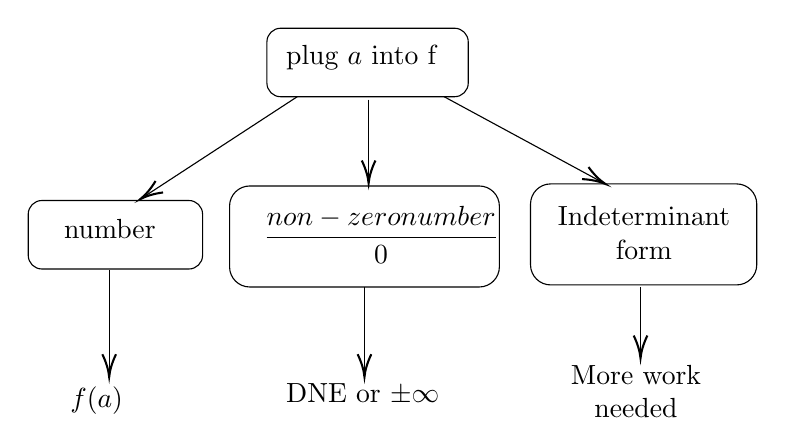
\begin{tikzpicture}[x=0.75pt,y=0.75pt,yscale=-1,xscale=1]
%uncomment if require: \path (0,446); %set diagram left start at 0, and has height of 446

%Rounded Rect [id:dp04536261924917495] 
\draw   (218,91.93) .. controls (218,88.29) and (220.95,85.33) .. (224.6,85.33) -- (308.4,85.33) .. controls (312.05,85.33) and (315,88.29) .. (315,91.93) -- (315,111.73) .. controls (315,115.38) and (312.05,118.33) .. (308.4,118.33) -- (224.6,118.33) .. controls (220.95,118.33) and (218,115.38) .. (218,111.73) -- cycle ;
%Straight Lines [id:da43038695232156465] 
\draw    (232.6,118.33) -- (158.67,166.57) ;
\draw [shift={(157,167.67)}, rotate = 326.87] [color={rgb, 255:red, 0; green, 0; blue, 0 }  ][line width=0.75]    (10.93,-3.29) .. controls (6.95,-1.4) and (3.31,-0.3) .. (0,0) .. controls (3.31,0.3) and (6.95,1.4) .. (10.93,3.29)   ;
%Straight Lines [id:da02535983624938165] 
\draw    (267,119.67) -- (267,158) ;
\draw [shift={(267,160)}, rotate = 270] [color={rgb, 255:red, 0; green, 0; blue, 0 }  ][line width=0.75]    (10.93,-3.29) .. controls (6.95,-1.4) and (3.31,-0.3) .. (0,0) .. controls (3.31,0.3) and (6.95,1.4) .. (10.93,3.29)   ;
%Straight Lines [id:da33645697944263864] 
\draw    (303.4,118.33) -- (379.24,159.38) ;
\draw [shift={(381,160.33)}, rotate = 208.42] [color={rgb, 255:red, 0; green, 0; blue, 0 }  ][line width=0.75]    (10.93,-3.29) .. controls (6.95,-1.4) and (3.31,-0.3) .. (0,0) .. controls (3.31,0.3) and (6.95,1.4) .. (10.93,3.29)   ;
%Rounded Rect [id:dp8149957234073693] 
\draw   (103,174.93) .. controls (103,171.29) and (105.95,168.33) .. (109.6,168.33) -- (180.4,168.33) .. controls (184.05,168.33) and (187,171.29) .. (187,174.93) -- (187,194.73) .. controls (187,198.38) and (184.05,201.33) .. (180.4,201.33) -- (109.6,201.33) .. controls (105.95,201.33) and (103,198.38) .. (103,194.73) -- cycle ;
%Rounded Rect [id:dp9518200785534192] 
\draw   (200,171.07) .. controls (200,165.69) and (204.36,161.33) .. (209.73,161.33) -- (320.27,161.33) .. controls (325.64,161.33) and (330,165.69) .. (330,171.07) -- (330,200.27) .. controls (330,205.64) and (325.64,210) .. (320.27,210) -- (209.73,210) .. controls (204.36,210) and (200,205.64) .. (200,200.27) -- cycle ;
%Rounded Rect [id:dp5380321492603661] 
\draw   (345,170.07) .. controls (345,164.69) and (349.36,160.33) .. (354.73,160.33) -- (444.27,160.33) .. controls (449.64,160.33) and (454,164.69) .. (454,170.07) -- (454,199.27) .. controls (454,204.64) and (449.64,209) .. (444.27,209) -- (354.73,209) .. controls (349.36,209) and (345,204.64) .. (345,199.27) -- cycle ;
%Straight Lines [id:da980017392599877] 
\draw    (142,202) -- (142,251.33) ;
\draw [shift={(142,253.33)}, rotate = 270] [color={rgb, 255:red, 0; green, 0; blue, 0 }  ][line width=0.75]    (10.93,-3.29) .. controls (6.95,-1.4) and (3.31,-0.3) .. (0,0) .. controls (3.31,0.3) and (6.95,1.4) .. (10.93,3.29)   ;
%Straight Lines [id:da24546083605149582] 
\draw    (265,210) -- (265,251.33) ;
\draw [shift={(265,253.33)}, rotate = 270] [color={rgb, 255:red, 0; green, 0; blue, 0 }  ][line width=0.75]    (10.93,-3.29) .. controls (6.95,-1.4) and (3.31,-0.3) .. (0,0) .. controls (3.31,0.3) and (6.95,1.4) .. (10.93,3.29)   ;
%Straight Lines [id:da8582799815353812] 
\draw    (398,210) -- (398,242.33) ;
\draw [shift={(398,244.33)}, rotate = 270] [color={rgb, 255:red, 0; green, 0; blue, 0 }  ][line width=0.75]    (10.93,-3.29) .. controls (6.95,-1.4) and (3.31,-0.3) .. (0,0) .. controls (3.31,0.3) and (6.95,1.4) .. (10.93,3.29)   ;

% Text Node
\draw (226,92.33) node [anchor=north west][inner sep=0.75pt]   [align=left] {plug $\displaystyle a$ into f};
% Text Node
\draw (119,176.33) node [anchor=north west][inner sep=0.75pt]   [align=left] {number};
% Text Node
\draw (355,170) node [anchor=north west][inner sep=0.75pt]   [align=left] {\begin{minipage}[lt]{65.09pt}\setlength\topsep{0pt}
\begin{center}
Indeterminant\\form
\end{center}

\end{minipage}};
% Text Node
\draw (122,256.83) node [anchor=north west][inner sep=0.75pt]   [align=left] {$f(a)$};
% Text Node
\draw (226,255.33) node [anchor=north west][inner sep=0.75pt]   [align=left] {DNE or $\displaystyle \pm \infty $};
% Text Node
\draw (361,246.33) node [anchor=north west][inner sep=0.75pt]   [align=left] {\begin{minipage}[lt]{50.33pt}\setlength\topsep{0pt}
\begin{center}
More work\\needed
\end{center}

\end{minipage}};
% Text Node
\draw (215,170) node [anchor=north west][inner sep=0.75pt]    {$\displaystyle\frac{\text{non-zero number}}{0}$};

\end{tikzpicture}
    }
    \caption{Flowchart for evaluating limits}
    \label{fig:flowchart}
\end{figure}

\subsection{A Number}

If $f$ is an ACCF and $f(a)$ is a number, then $a$ is in the domain of $f$. Since any ACCF is continuous on its domain,
$$\lim_{x\to a}f(x)=f(a)$$
by the definition of continuity. \mar{Re-read this until you understand it!}

\subsection{A (non-zero) Number over Zero}

If $f$ is an ACCF and attempting to evaluate $f(a)$ results in a non-zero number over 0, then $f$ has a vertical asymptote at $x=a$. Near $x=a$, the values of $f(x)$ get very close to either positive or negative infinity. The right and left sided limits are either positive or negative infinity, so there are only four cases, as seen in figure \ref{fig:four-cases}.

\begin{figure}[h]
    \centering
    \fbox{
        \resizebox{4.25in}{!}{
        \tikzset{every picture/.style={line width=0.75pt}} %set default line width to 0.75pt        
        
        \begin{tikzpicture}[x=0.75pt,y=0.75pt,yscale=-1,xscale=1]
        %uncomment if require: \path (0,446); %set diagram left start at 0, and has height of 446
        
        %Straight Lines [id:da7130638550602129] 
        \draw    (17.32,128.98) -- (162.73,128.98) ;
        %Curve Lines [id:da8198586763402247] 
        \draw    (19.1,124.51) .. controls (81.55,124.51) and (86.01,102.21) .. (86.01,57.6) ;
        %Curve Lines [id:da33054163491632704] 
        \draw    (161.84,124.51) .. controls (99.39,124.51) and (94.93,102.21) .. (94.93,57.6) ;
        %Straight Lines [id:da39635263385432795] 
        \draw  [dash pattern={on 0.84pt off 2.51pt}]  (90.47,54.93) -- (90.47,201.24) ;
        
        %Straight Lines [id:da4984898910131832] 
        \draw    (187.51,128.98) -- (332.93,128.98) ;
        %Curve Lines [id:da12653349982399664] 
        \draw    (189.3,124.51) .. controls (251.75,124.51) and (256.21,102.21) .. (256.21,57.6) ;
        %Curve Lines [id:da6963380775085903] 
        \draw    (332.04,133.14) .. controls (269.59,133.14) and (265.13,155.74) .. (265.13,200.05) ;
        %Straight Lines [id:da5434138892345324] 
        \draw  [dash pattern={on 0.84pt off 2.51pt}]  (260.67,54.93) -- (260.67,201.24) ;
        
        %Straight Lines [id:da6992946751383504] 
        \draw    (357.71,128.98) -- (503.13,128.98) ;
        %Curve Lines [id:da5321156852218221] 
        \draw    (359.5,132.54) .. controls (421.95,132.54) and (426.41,155.74) .. (426.41,200.05) ;
        %Curve Lines [id:da8818577355654187] 
        \draw    (502.24,124.51) .. controls (439.79,124.51) and (435.33,102.21) .. (435.33,57.6) ;
        %Straight Lines [id:da23325172919339887] 
        \draw  [dash pattern={on 0.84pt off 2.51pt}]  (430.87,54.93) -- (430.87,201.24) ;
        
        %Straight Lines [id:da2808110791577314] 
        \draw    (527.91,128.98) -- (673.33,128.98) ;
        %Curve Lines [id:da43641618110544544] 
        \draw    (530,133.73) .. controls (592.45,133.73) and (596.91,155.14) .. (596.91,200.05) ;
        %Curve Lines [id:da16583705050218067] 
        \draw    (672.44,133.14) .. controls (609.99,133.14) and (605.53,155.74) .. (605.53,200.05) ;
        %Straight Lines [id:da9264659475889601] 
        \draw  [dash pattern={on 0.84pt off 2.51pt}]  (601.07,54.93) -- (601.07,201.24) ;
        
        
        
        
        
        \end{tikzpicture}
        
        % \resizebox{3in}{!}{
        % \tikzset{every picture/.style={line width=0.75pt}} %set default line width to 0.75pt        
        % \begin{tikzpicture}[x=0.75pt,y=0.75pt,yscale=-1,xscale=1]
        % %uncomment if require: \path (0,446); %set diagram left start at 0, and has height of 446
        
        % %Straight Lines [id:da11666177611802953] 
        % \draw    (98,120.33) -- (261,120.33) ;
        % %Curve Lines [id:da20823749405635383] 
        % \draw    (100,115.33) .. controls (170,115.33) and (175,90.33) .. (175,40.33) ;
        % %Curve Lines [id:da5857981133236727] 
        % \draw    (260,115.33) .. controls (190,115.33) and (185,90.33) .. (185,40.33) ;
        % %Straight Lines [id:da8270643292998765] 
        % \draw  [dash pattern={on 0.84pt off 2.51pt}]  (180,37.33) -- (180,201.33) ;
        
        % %Straight Lines [id:da6737028355731796] 
        % \draw    (288,120.33) -- (451,120.33) ;
        % %Curve Lines [id:da5853120673537593] 
        % \draw    (290,115.33) .. controls (360,115.33) and (365,90.33) .. (365,40.33) ;
        % %Curve Lines [id:da33546715055487053] 
        % \draw    (450,125) .. controls (380,125) and (375,150.33) .. (375,200) ;
        % %Straight Lines [id:da39333458455778736] 
        % \draw  [dash pattern={on 0.84pt off 2.51pt}]  (370,37.33) -- (370,201.33) ;
        
        
        % %Straight Lines [id:da41843468171367526] 
        % \draw    (98,310.33) -- (261,310.33) ;
        % %Curve Lines [id:da9482877395734075] 
        % \draw    (100,314.33) .. controls (170,314.33) and (175,340.33) .. (175,390) ;
        % %Curve Lines [id:da7803855380541431] 
        % \draw    (260,305.33) .. controls (190,305.33) and (185,280.33) .. (185,230.33) ;
        % %Straight Lines [id:da11027576459803168] 
        % \draw  [dash pattern={on 0.84pt off 2.51pt}]  (180,227.33) -- (180,391.33) ;
        
        % %Straight Lines [id:da294114983098098] 
        % \draw    (288,310.33) -- (451,310.33) ;
        % %Curve Lines [id:da491751074451225] 
        % \draw    (290.33,315.67) .. controls (360.33,315.67) and (365.33,339.67) .. (365.33,390) ;
        % %Curve Lines [id:da32646541541064433] 
        % \draw    (450,315) .. controls (380,315) and (375,340.33) .. (375,390) ;
        % %Straight Lines [id:da20001269749677508] 
        % \draw  [dash pattern={on 0.84pt off 2.51pt}]  (370,227.33) -- (370,391.33) ;
        
        
        
        
        
        
        % \end{tikzpicture}
        % }
        }
    }
    \caption{The four cases of vertical asymptotes}
    \label{fig:four-cases}
\end{figure}

Therefore, the only possibilities for the value of these limits are $\infty$, $-\infty$, and DNE. \mar{Label each function in figure \ref{fig:four-cases} with its respective limit.} To figure it out which one it is, evaluate both of the two sided limits. For each, plug in a value that is slightly to the right (or the left) of $a$. If the result is positive, the sided limit is positive infinity, and if the result is negative, negative infinity.

\subsection{Indeterminant Form}

There are seven indeterminant forms:

\vspace{1em}

\begin{center}
\begin{Large}
\phantom{}\hfill
$\frac{0}{0}$ \hfill
$\frac{\infty}{\infty}$ \hfill
$0^0$ \hfill
$\infty{-}\infty$ \hfill
$1^\infty$ \hfill
$0{\cdot}\infty$ \hfill
$\infty^0$
\hfill\phantom{}
\end{Large}
\end{center}

\vspace{1em}

They are called \textbf{indeterminant} because in this form, we cannot be sure of its value (or even if its value makes sense). Take $0^0$ for example: zero raised to any power should be 0, but anything raised to the power of $0$ should be 1... so which is it? \mar{Write out similar question for the other 6 indeterminant forms.}

When we get an indeterminant form after trying to evaluate $f(a)$, we need to do more work. There are several things you can try:

\begin{itemize}
\item Simplify. If the function is rational and has common factor in its numerator and denominator, by ``canceling'' the term, the resulting function is not the same: the original function has a hole at the point where the factored term is 0. For example, $f(x)=\frac{x(x-1)}{(x-1)}$ has a hole at $x=1$, but everywhere else is the line $y=x$. However, this cancellation does not change the value of the limit.
\item Multiply the numerator and denominator of a rational function by the conjugate of the denominator or the numerator (the \textbf{conjugate} of a binomial $a+b$ is $a-b$).
\item Use a special-case limit: 
$$
\lim_{x\to 0}\frac{\sin(x)}{x} = 1
\quad\quad\quad\quad
\lim_{x\to 0}\frac{\cos(x) - 1}{x} = 0
$$
$$
\lim_{x\to\infty}\left(1+\frac{1}{x}\right)^x = e
\quad\quad\quad\quad
\lim_{x\to 0}\frac{a^x-1}{x}=\ln(a)
$$

\item In the case of $x\to\pm\infty$ for a rational function, divide the numerator and denominator by the highest degree term of the denominator.

\item Use the Squeeze Theorem:

\begin{thm}[Squeeze Theorem]
Let $f$, $g$, and $h$ be functions with $g(x)\leq f(x)\leq h(x)$ for all $x$ in some interval around $a$ (except possibly at $a$). If $$\lim_{x\to a}g(x)=L=\lim_{x\to a} h(x),$$ then $$\lim_{x\to a} f(x)=L$$
as well.
\end{thm}
The most common application of squeeze theorem is squeezing $$-1\leq \sin\theta \leq 1.$$

\end{itemize}

Later, we will learn a trick called L'H\^opital's Rule to more easily compute limits with indeterminant forms. But first we need to learn about derivatives!












